\chapter{Defeasible Reasoning}
\label{chapter:defeasible-reasoning}

Non-monotonicity in logical systems has been the focus of study for decades, and several distinct formalisms have been developed. The
motivation is to expand the inference power beyond that of the classical, to a more credulous one. This work is primarily interested in non-monotonic
reasoning following the preferential semantics introduced by Shoham \cite{shohamSemanticApproach}, for which there is a well-developed model
theory which further benefits from an obvious analogue to notions central to FCA. In particular, we are interested in the framework put forward
by Kraus, Lehmann, and Magidor \cite{kraus1990nonmonotonic,lehmann1992what}, frequently initialised to the `KLM framework'.

In the proceeding, we provide a background on non-monotonic reasoning in general, before introducing the KLM framework. We assume all the same
conventions introduced in \Cref{section:propositional-logic} for the technical discussions which occur in this chapter.

\section{Background on Non-monotonic Reasoning}
\label{section:nmr-background} Near the end of the previous chapter, the matter of consequence was discussed in a very formal sense. It is perhaps
helpful to distinguish this subject---classical consequence---from the common concept, as the former yields some surprising results which do
not appear at all congruent with how a person, or otherwise intelligent agent should reason \cite{tarski1936consequence, kraus1990nonmonotonic}.
For a demonstration of a result which may be \textit{surprising} in this way, consider the following propositions:
\vspace{1em}
\begin{enumerate}
  \item $\texttt{human}\rightarrow \texttt{chronological time}$

  \item $\texttt{soldier}\rightarrow \texttt{human}$

  \item $\texttt{billy pilgrim}\rightarrow \neg \texttt{chronological time}$
\end{enumerate}
\vspace{1em}

Knowing these propositions, if we were to encounter an individual in fatigues we might find it sensible---by propositions 2 and 1---to infer
that the individual experienced time chronologically. If we were to later learn that the individual was, in fact, Billy Pilgrim, given proposition
3, we should like to retract our prior inference, replacing it with the knowledge that the individual does not experience time chronologically.

Such recourse is not, as it stands, possible: When we see the that the individual is a soldier, the possible worlds satisfying our knowledge
are reduced to the single model: $\{\overline{b},c,h,s\}$ (where $b$: \texttt{billy pilgrim}, $c$: \texttt{chronological time}, $h$: \texttt{human},
and $s$: \texttt{soldier}). Should we later learn that the individual is indeed Billy Pilgrim, the theory becomes inconsistent.
%TODO: Add section in preliminaries about principle of explosion
And, by the principle of explosion, discussed in \Cref{subsection:logical-consequence}, our theory now entails that the individual experiences
time both chronologically and non-chronologically; indeed our theory entails everything and is accordingly worthless.

This property of classical logic---that adding new information never results in retraction of pre-existing knowledge---is called
monotonicity. Monotonicity requires that when we make a claim like \say{humans experience time chronologically}, we must be absolutely sure of
ourselves, so as to never worry about needing to retract an inference. This is, of course, too strict a requirement as we cannot determine for
all future, present, and past humans if it were the case that they experienced time chronologically. If we remain in the classical realm, it
seems our only options are to abandon our original claim or risk explosion.

At this point it is a good idea to provide some clarification on how we might begin to approach this issue. Continuing with the same example---and
continuing to allow ourselves to entertain the possibility of experiencing non-chronological time---it would certainly be agreed that
typically soldiers are human, and also that typically humans experience time chronologically. To resolve that Billy Pilgrim is a soldier, and
therefore a human, who does not experience chronological time, we need only to point out that he is an atypical human.

To make the previous paragraph more formal, we remind the reader of the discussion held around \Cref{definition:logical-consequence}: A formula
$\phi$ is a logical consequence of a set $\Gamma$ thereof if every model of $\Gamma$ is also a model of $\phi$. Put differently, there is no
valuation (or, possible world) where $\Gamma$ is true and $\phi$ is false. It follows directly that $\phi$ remains a logical consequence of $\Gamma
\cup \{\psi\}$, since $\Gamma$ is true in any world where $\Gamma \cup \{\psi\}$ is true.

It was pointed out by Shoham \cite{shohamSemanticApproach} that we may \say{bend the rules} and restrict semantic consideration to a privileged
subset of models deemed ``preferable''. We call these selected models the ``minimal'' models---a choice that will become clearer as this
chapter progresses.

% \section{Preferential Reasoning}
% \label{section:preferential-reasoning}
% In this work we are interested specifically in the KLM-style of non-monotonic reasoning, which will be introduced in the proceeding chapter. As a precursor, it is beneficial to discuss the semantic approach to non-monotonic reasoning put forward by Shoham \cite{shohamSemanticApproach}.

% \begin{definition}
% \label{definition:preferential-satisfaction-from-valuation}
% Given a formula $\phi \in \mathcal{L}$ and a valuation $u \in \mathcal{U}$, then $u$ \emph{preferentially satisfies} $\phi$ (and we write $u \vDash_\sqsubseteq \phi $) if and only if there is no other interpretation $v \in \mathcal{U}$ where $v \vDash \phi$ and $v \sqsubset u$. Then $u$ is a \emph{preferred}, or \emph{minimal} model of $\phi$.
% \end{definition}

% \begin{definition}
% \label{definition:preferential-satisfiability}
% A formula $\phi \in \mathcal{L}$ is \emph{preferentially satisfiable} if it has a preferred model.
% \end{definition}

% From the two definitions above it may be obvious that every preferentially satisfiable formula is indeed classically satisfiable, while the converse is not true: To see why we need only consider an infinitely descending chain of valuations, and whether a tautology is preferentially satisfiable in such a structure.
\section{The KLM Framework}
The KLM framework for non-monotonic reasoning was initially described by a collection of consequence relations satisfying certain axioms---frequently
called the \textit{rationality postulates}---with each successive system being stronger than its predecessor. We borrow a nice story from Dov
Gabbay \cite{gabbay1985theoreticalFoundations} which motivates why consequence relations are a good starting point for the study of a non-monotonic
system.

Paraphrasing, he begins by asking the reader to imagine a machine that does non-monotonic inference in some domain. The machine represents knowledge
as formulae and so we pose queries of the form \say{Does $\psi$ non-monotonically follow from $\phi$?}. Something goes awry (suppose some
coffee was spilled), calling into question whether the logic of the machine still functions correctly. Even worse, the interface, which tells
us what real-world instance each formula maps to, is destroyed and so function cannot be evaluated based on the meaning of the formulae the
machine reasons on. How might we then evaluate the machine's function?

If we were interested in classical consequence, we would be well-equipped to assess the correctness of the machine by determining if it
satisfied reflexivity, monotonicity, and cut (we point to \Cref{definition:consequence-relations} as a reminder). This is precisely the starting
point that Kraus, Lehmann, and Magidor took up in \cite{kraus1990nonmonotonic}, suggesting that before getting to the semantics of a non-monotonic
system, it is a good idea to formalise axiomatise the system as a consequence relation satisfying certain properties.

The rationality postulates are precisely this axiomatisation, characterising a sensible pattern of reasoning for non-monotonic systems. We use
`$\twiddle$' (pronounced ``twiddle'') instead of `$\vdash$' to denote a non-monotonic consequence relation. As we may expect, $\phi \twiddle
\psi$ has the same meaning as $(\phi, \psi) \in \; \twiddle$, and $\phi \ntwiddle \psi$ as $(\phi, \psi)\not \in \; \twiddle$. We may, at
times of potential confusion, use a subscript to disambiguate which consequence relation is being referred to, and so $\twiddle_{C}$ would
refer to a cumulative relation, as defined below.

% An expression like $\phi \twiddle \psi$ is to be understood as saying \say{If $\phi$ holds, then $\psi$ is a typical consequence}, we call
% expressions of this nature \textit{conditional assertions}. The properties that a particular consequence relation satisfies are represented
% as rules of inference in the style of conditional assertions.

\subsection{Cumulative Reasoning}
\label{subsection:system-c}

\textit{Cumulative consequence relations}, otherwise referred to as \textit{System C}, represent the weakest of the systems in the KLM framework.
We follow the same exposition, from weaker to stronger systems, as \cite{kraus1990nonmonotonic}: this approach will minimise repetition, as
each successive system inherits all properties of its predecessor.

\begin{definition}
  \label{definition:cumulative-consequence-relation} A consequence relation $\twiddle$ is a \emph{cumulative consequence relation} if and
  only if it satisfies the properties of \emph{Reflexivity, Left Logical Equivalence, Right Weakening, Cut} and \emph{Cumulative
  Monotonicity}.
\end{definition}

The first axiom, \textit{Reflexivity}, is largely self justifying: It makes little sense to speak about a notion of consequence that does not
satisfy this property.

\begin{align}
  \label{postulate:ref}\inferLeft{Reflexivity}{}{\phi \twiddle \phi}
\end{align}

The justification for \textit{Left Logical Equivalence} is a bit more opaque; the principle is that if two scenarios represent the same
state of affairs, and in one of these scenarios it we typically expect some consequence, then we should expect the same in the other
scenario.

\begin{align}
  \label{postulate:lle}\inferLeft{Left Logical Equivalence}{\vdash \phi \leftrightarrow \psi, \quad \phi \twiddle \gamma}{\psi \twiddle \gamma}
\end{align}

\textit{Right Weakening} allows the preservation of classical consequence within the logic. It says that if it is always the case that from knowing
$\psi$ we conclude $\gamma$, and from knowing $\phi$ we normally conclude $\psi$, then we are entitled to hold the view that from $\phi$ we normally
expect $\gamma$ as well.

\begin{align}
  \label{postulate:rw}\inferLeft{Right Weakning}{\vdash \psi \rightarrow \gamma, \quad \phi \twiddle \psi}{\phi \twiddle \gamma}
\end{align}

\textit{Cautious Monotony} (which has also be called \textit{Cumulative Monotony} by Makinson \cite{makinson2003bridges}, and \textit{Restricted
Monotony} by Gabbay \cite{gabbay1985theoreticalFoundations}) corresponds to the notion that if we are in an epistemic state $\phi$ where one
expectation, among others, is that $\psi$ holds. Learning that $\psi$ indeed holds should not alter the epistemic state in such a way that the
\textit{other} expectations are abandoned, and so the new state, $\phi \land \psi$, we should expect everything that was expected when all we
knew was $\phi$. In other words, we reason monotonically with respect to expected information.

\begin{align}
  \label{postulate:cm}\inferLeft{Cautious Monotony}{\phi \twiddle \psi, \quad \phi \twiddle \gamma }{\phi \land \psi \twiddle \gamma}
\end{align}

Certain other rules may derived from the presence of already discussed postulates. A version of \textit{Cut}

\begin{align}
  \label{postulate:cut}\inferLeft{Cut}{\phi \land \psi \twiddle \gamma, \quad \phi \twiddle \psi}{\phi \twiddle \gamma}
\end{align}

The original version due to Gentzen \cite{Ben1993Mathematical} is presented as:
\begin{align}
  \inferLeft{Monotonic Cut}{\phi \land \psi \twiddle \gamma, \quad \alpha \twiddle \psi}{\phi \land \alpha \twiddle \gamma}
\end{align}
implies monotonicity, as it requires that if $\psi$ is a typical consequence of $\alpha$, then it must remain a consequence of $\alpha \land
\phi$: ergo, monotonicity. The former variation does not enforce this, and rather says \say{Suppose I have certain knowledge of $\phi$, and that if I were to assume $\psi$ I should expect to conclude $\gamma$. Then if I can show that infact $\psi$ was already an expected consequence of knowing $\phi$, I should expect that $\gamma$ follows from $\phi$}.
When considered alongside the argument for Cautious Monotony, Cut seems obviously acceptable.

The \textit{And} postulate suggests that if $\psi$ and $\gamma$ are both expected consequence of $\phi$, then their conjunction is also
expected. This postulate fails in probabilistic systems, such as \textit{association rules} \cite{gabbay1985theoreticalFoundations}.
\begin{align}
  \label{postulate:and}\inferLeft{And}{\phi \twiddle \psi, \quad \phi \twiddle \gamma}{\phi \twiddle \psi \land \gamma}
\end{align}

The following Lemma is a helpful intuition pump, it is largely why the term \textit{cumulative} is used for this system: it suggests that we
can use the consequences of plausible inferences to make further plausible inferences.
\begin{lemma}
  \label{lemma:cut-cautious} We can cover the properties of \emph{Cut} and \emph{Cumulative Monotonicity} with the following principle: \say{If $\phi \twiddle \psi$, then the typical consequences of $\phi$ and $\phi \land \psi$ coincide}.
\end{lemma}

Certain, frequently discussed properties in classical logic do not hold in cumulative consequence relations. Most obviously, cumulative consequence
relations do not satisfy
\begin{align}
  \label{postulate:monotonicity}\inferLeft{Monotonicity}{\psi \rightarrow \gamma, \quad \gamma \twiddle \phi}{\psi \twiddle \phi}
\end{align}
In addition, \textit{Transitivity} and \textit{Contraposition} which both imply monotonicity when considered alongside the other rules of
cumulative relations
\begin{align}
  \label{postulate:trans}\inferLeft{Transitivity}{\phi \twiddle \psi, \quad \psi \twiddle \gamma}{\phi \twiddle \gamma}
\end{align}
Transitivity, in \Cref{proof:transitivity}, was shown to be quite useful as a derived rule of a Hilbert system; but, for our purposes, it will
not do. Consider the example at the beginning of this chapter, where the topic of whether we should infer that Billy Pilgrim experiences chronological
time. Transitivity requires that we infer he does: Billy Pilgrim is a soldier, soldiers are human, and humans experience time chronologically.
But this is precisely the inference we do not want, and so transitivity must be abandoned.
%
\begin{align}
  \label{postulate:contra}\inferLeft{Contraposition}{\phi \twiddle \psi}{\neg \psi \twiddle \neg \phi}
\end{align}

These properties are undesirable as they imply monotonicity, precisely what we are interested in avoiding. However, it is worth reminding
ourselves of the discussion at the beginning of this chapter: That our aim is to develop a system which allows for more (credulous) inferences
to be made. A question that arises is whether non-monotonic systems should be \textit{supraclassical} \cite{makinson2003bridges}: should
classical inferences be preserved? Under the framing we have adopted, that classical deductions require iron-clad proofs beyond which is
often practical, and that these requirements could be relaxed in order to make more useful (but retractable) inferences. Then, if we have a classical
proof of something it should of course hold in a non-monotonic system.

\begin{align}
  \label{postulate:supraclassical}\inferLeft{Supraclassical}{\phi \rightarrow \psi}{\phi \twiddle \psi}
\end{align}

\textcolor{red}{Diagram ovals of worlds}

We will skip over any discussion of semantics for cumulative consequence relations, and rather opt to introduce these in the next section where
we discuss preferential consequence relations.

\subsection{Preferential Reasoning}
\label{subsection:system-P}

We, quite quickly, move on from cumulative to \textit{preferential consequence relations}, or \textit{system P}. The reason being that
system P is strictly stronger than system C, and includes in its' axiomatisation something analogous to the more significant part of the
deduction theorem, as well as disjunction. The semantics of system P, to be outlined in \Cref{subsubsection:preferential-interpretations},
are similar to the approach which was proposed by Shoham in \cite{shohamSemanticApproach}.

Fortunately, the definition of a preferential consequence relation is almost identical to that of cumulative one, with only the addition of
the \textit{Or} postulate.

\begin{definition}
  \label{definition:preferential-relation} The consequence relation $\twiddle$ is a \emph{preferential consequence relation} if and only if
  it satisfies the properties of \emph{Reflexivity, Left Logical Equivalence, Right Weakening, Cut, Or,} and \emph{Cumulative Monotonicity}.
\end{definition}

As a justification for \textit{Or}, consider that \textit{If Billy were abducted by aliens, normally he would be traumatised}, but also
\textit{If Billy witnessed the fire-bombing of Dresden, normally he would be traumatised}. If we know that at least one of these events
happened we should be allowed to conclude that Billy were traumatised, since either of them would normally allow this inference.

\begin{align}
  \inferLeft{Or}{\phi \twiddle \gamma, \quad \psi \twiddle \gamma}{\phi \lor \psi \twiddle \gamma}
\end{align}

The addition of \textit{Or} to the rest of the properties of system C allow for useful derived rules. For instance, \textit{S}

\begin{align}
  \inferLeft{S}{\phi \land \psi \twiddle \gamma}{\phi \twiddle \psi \rightarrow \gamma}
\end{align}

The derived rule \textit{S} is analogous to the deduction theorem (cf. \Cref{axiom:deduction-theorem}), and

\begin{lemma}[\cite{shohamSemanticApproach}]
  For $\phi, \psi \in \mathcal{L}$ and some valuation $u \in \mathcal{U}$, if $u \vdash \psi$ and $u \twiddle \phi$, then $u \twiddle \phi \land
  \psi$.
\end{lemma}

\subsubsection{Preferential Interpretations}
\label{subsubsection:preferential-interpretations}

In this account of the semantics of system P, our aim is to construct

In this account of the semantics of preferential systems, it is our aim to construct more-or-less full correspondence between the tools we have
available in the model theory of propositional logic, and the model theory of preferential systems. Accordingly, it will be helpful to
recall some basic terminology from \Cref{section:propositional-logic}: A \textit{model} of a formula $\phi$ (set of formulae) is a valuation
$v$ that satisfies it, and we write $v \vDash \phi$. A formula $\phi$ is \textit{satisfiable} if it has a model, and \textit{valid} if every
possible valuation is a model of $\phi$. A formula $\psi$ is a logical consequence of another $\phi$ if all models of $\phi$ are
additionally models of $\psi$, and we write $\phi \vDash \psi$.

A semantics for preferential systems can be constructed by equipping the set of all valuations $\mathcal{U}$ with a preference relation, and
then restricting ones consideration from all models of a formula to only those \textit{preferred} models.

\begin{definition}
  \label{definition:preferential-interpretation} A \emph{preferential interpretation} $W$ is a triple $(S, l, \prec)$ where $S$ is a set of
  \emph{states}, $l: S \mapsto \mathcal{U}$ is a function mapping states to valuations, and $\prec$ is a strict partial-order on $S$.
\end{definition}

\begin{definition}
  \label{definition:state-satisfaction} In a preferential interpretation $W$, we say that a state $s \in S$ \emph{satisfies} a formula $\phi
  \in \mathcal{L}$ if and only if the valuation $l(s) \vDash \phi$. For brevity, we write $s \VDash \phi$, and denote the set of all states
  satisfying $\phi$ by $\hat{\phi}$.
\end{definition}

\begin{definition}
  \label{definition:state-minimal} Given a preferential interpretation $W$ and formula $\phi \in \mathcal{L}$, we write $\hat{\phi}$ to
  denote the set $\{s \VDash \phi \mid s \in S\}$ of all states that satisfy $\phi$. We write $\underline{\hat{\phi}}$ to denote the set $\{s
  \in \hat{\phi}\mid \nexists s' \in \hat{\phi}\text{ such that }s' \prec s \}$ of $\prec$-\textit{minimal} states.
\end{definition}

\begin{example}
  \label{example:preferential-interpretation}

  Consider a knowledge base $\{h \twiddle c, \; s \twiddle h, \; b \rightarrow \neg c\}$ telling us that \say{Normally, humans experience chronological time},
  \say{Normally, soldiers are human}, and \say{Billy Pilgrim experiences non-chronological time}.

  \Cref{figure:preferential-interpretation} demonstrates a possible preferential interpretation of the knowledge base: each set represents
  the set of all states which witness the propositional atoms, and so a state in the green shaded area corresponds to one that satisfies $b,s
  ,h$ but not $c$.

  \begin{figure}[H]
    \centering
    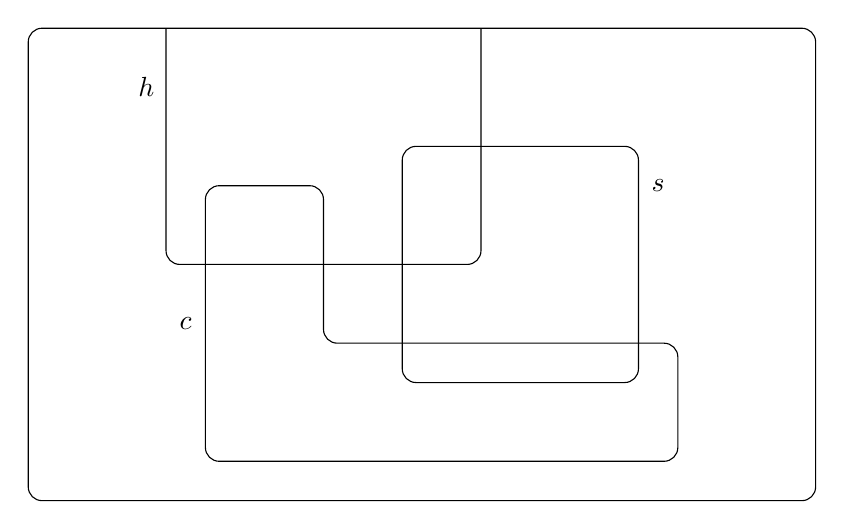
\begin{tikzpicture}
      % outer frame
      % \draw[help lines] (0,0) grid (10,6);
      \draw[rounded corners=5pt] (0,0) rectangle (10,6);

      % translate all three shapes at once
      \begin{scope}[shift={(0.75,0)}]
        % shape 1: HUMANS
        % \filldraw[rounded corners=5pt, fill=blue, fill opacity=0] (1,6) rectangle (5,3);
        \node (human) at (0.75,5.25) [] {$h$};
        \draw[rounded corners=5pt] (1,6) -- (1,3) -- (5,3) -- (5,6);

        % % shape 2: CHRONOLOGICAL
        \filldraw[rounded corners=5pt, fill=red, fill opacity=0] (1.5,4) -- (3,4) -- (3,2) -- (7.5,2) -- (7.5,0.5) -- (1.5,0.5) -- cycle;
        %   (1.5,3.25) --
        %   (3,3.25) --
        %   (3,1.75) --
        %   (6.5,1.75) --
        %   (6.5,0.25) --
        %   (1.5,0.25) --
        %   cycle;
        \node (chronological) at (1.25,2.25) [] {$c$};

        % % shape 3: SOLDIER
        \filldraw[rounded corners=5pt, fill=green, fill opacity=0] (4,4.5) -- (7,4.5) -- (7,1.5) -- (4,1.5) -- cycle;
        %   (3.75,3) --
        %   (3.75,4.5) --
        %   (8,4.5) --
        %   (8,1) --
        %   (5.5,1) --
        %   (5.5,3) --
        %   cycle;
        \node (soldier) at (7.25,4) [] {$s$};

        % % shape 4: BILLY
        % \filldraw[rounded corners=5pt, fill=green, fill opacity=0] (3,4.25) -- (4.5,4.25) -- (4.5,3.75) -- (3,3.75) -- cycle;
        % \node (billy) at (2.75,4.25) [] {$b$};

        % % % overlap of shape 1 & shape 2: dots
        % \begin{scope}
        %   \clip[rounded corners=5pt] (0.5,5) rectangle (4.5,1.75);
        %   \clip[rounded corners=5pt] (1.5,3.25) -- (3,3.25) -- (3,1.75) -- (6.5,1.75) -- (6.5,0.25) -- (1.5,0.25) -- cycle;
        %   \fill[pattern=dots, pattern color=red] (0,0) rectangle (10,6);
        % \end{scope}

        % \begin{scope}
        %   % clip to human rectangle
        %   \clip[rounded corners=5pt] (0.5,5) rectangle (5,2.5);
        %   % clip to soldier L-shape
        %   \clip[rounded corners=5pt] (3.75,3) -- (3.75,4.5) -- (8,4.5) -- (8,1) -- (5.5,1) -- (5.5,3) -- cycle;
        %   % fill their intersection with blue dots
        %   \fill[pattern=dots, pattern color=blue] (0,0) rectangle (10,6);
        % \end{scope}

        % % overlap of BILLY and SOLDIER: green hatch
        % \begin{scope}
        %   % clip to BILLY’s tiny rectangle
        %   \clip[rounded corners=5pt] (3,4.25) -- (4.5,4.25) -- (4.5,3.75) -- (3,3.75) -- cycle;
        %   % clip to SOLDIER’s L–shape
        %   \clip[rounded corners=5pt] (3.75,3) -- (3.75,4.5) -- (8,4.5) -- (8,1) -- (5.5,1) -- (5.5,3) -- cycle;
        %   % fill their intersection with green lines
        %   \fill[pattern=north east lines, pattern color=green] (0,0) rectangle (10,6);
        % \end{scope}
      \end{scope}
    \end{tikzpicture}
    \caption{A preferential interpretation}
    \label{figure:preferential-interpretation}
  \end{figure}
\end{example}

\begin{definition}
  \label{definition:preferential-satisfaction} A preferential interpretation $W$ \emph{satisfies} a defeasible conditional
  $\phi \twiddle \psi$ if and only if the $\prec$-\emph{minimal} states which satisfy $\phi$ also satisfy $\psi$, equivalently if
  $W \vDash_{P}\phi \twiddle \psi$ if $\underline{\hat{\phi}}\subseteq \hat{\psi}$.
\end{definition}

\begin{definition}
  \label{definition:preferentially-satisfiable} A formula $\phi \in \mathcal{L}$ is \emph{preferentially satisfiable} if and only if there
  exists a preferential interpretation $W$ such that $W\vDash_{P}\phi$
\end{definition}

\begin{theorem}[Soundness]
  \label{theorem:soundness-preferential} If $W$ is a preferential interpretation which defines the consequence relation $\twiddle_{W}$, then
  $\twiddle_{W}$ satisfies \textit{Reflexivity, Left Logical Equivalence, Right Weakening, Or,} and \textit{Cautious Monotony}.
\end{theorem}

\begin{theorem}[Completeness]
  \label{theorem:completeness-preferential} If $\twiddle_{P}$ is a preferential consequence relation, then there exists a preferential
  interpretation $W$ which induces the consequence relation $\twiddle_{W}$ such that $\twiddle_{P}$ is precisely $\twiddle_{W}$.
\end{theorem}

\subsection{Preferential Entailment}

RE iT not being nmr We are willing to accept these credulous inferences precisely because they may be retracted we may withdraw previous
inferences under learning new facts.

\section{Rational Closure}

\subsection{Rational Consequence Relations}